% Context, isothermal, thermodynamical framework, standard generalized material etc.
In this section, the mathematical laws allowing the description of the deformation of a solid body will be derived. First, the kinematic laws governing the motion of each material point belonging to a solid will be considered. The variations of lengths and shapes of a continuum, described by the \textit{strain} mesure will then be associated to internal forces through thermodynamic framework. Finally, the theory of first order quasi-linear partial differential system will be applied to solid dynamics in order to deliver analytical solutions for specific problems.

\subsection{Kinematic laws}
We consider a three-dimensional solid domain bounded by a volume denoted by $\Omega \in \Rbb^3$. This body undergoes external sollicitations that can either be localized on a part of the external surface of the body (\textit{i.e. surface forces}) or act in the whole solid domain (\textit{i.e. volume forces}). Due to the presence of such sollicitations, the volume may change during a deformation within the time interval $\tau = \[0,T\]$ and will hence be written as a function of time $\Omega(t)$ ($t\in \tau$). The state of the solid at time $t=0$, corresponding to a non-deformed state with volume $\Omega(t=0)=\Omega_0$, is referred to as the \textit{initial configuration}. Some problems require the use of a \textit{reference configuration} that can be deformed and to which equations are referred. In what follows, the reference and initial conditions are identical. At a given time $t>0$, the volume $\Omega(t)=\Omega_t$ corresponds to the \textit{current configuration}. These configurations are depicted in figure \ref{fig:deformationFunction}.
\begin{figure}[h]
  \centering
  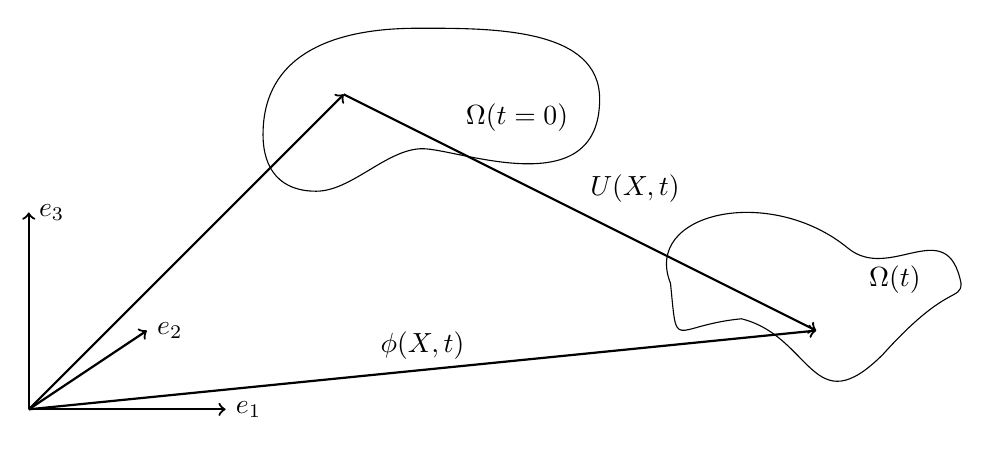
\begin{tikzpicture}
  %\draw[step=1.0,black,thin] (-3.,-1.) grid (3,4.);
  %\draw (-3,-1) -- (3,-1) -- (3,4) -- (-3,4) -- (-3,-1);
  \draw[thick,->] (-5,-2.5) -- (-2.5,-2.5) node [right] {$\vect{e}_1$};
  \draw[thick,->] (-5,-2.5) -- (-5,0.) node [right] {$\vect{e}_3$};
  \draw[thick,->] (-5,-2.5) -- (-3.5,-1.5) node [right] {$\vect{e}_2$};
  \begin{scope}[scale=0.45]
    \draw (-3,0.6) .. controls +(1,0) and +(-1,0) .. (0,1.8)  
    .. controls +(1,0) and +(0,-3) .. (5,3.2) 
    .. controls +(0,2) and +(2,0)  .. (0,5.2) 
    .. controls +(-1,0) and +(0,3) .. (-4.5,2.2) 
    .. controls +(0,-1) and +(-1,0).. (-3,0.6) ;
  \end{scope}
  \node at (1.2,1.2) {$\Omega(t=0)$};
  %% Deformed body +2.
  \begin{scope}[scale=0.9]
    \draw (0.+0.5+4.,0-1.5) ..controls (1.+0.5+4.,-0.25-1.5) and (1.+0.5+4.,-1.5-1.5) .. (2.+0.5+4.,-0.5-1.5) ..controls (2.9+0.5+4.,0.5-1.5) and (3.1+0.5+4.,0.25-1.5) .. (3.1+0.5+4.,0.5-1.5) ..controls (2.9+0.5+4.,1.5-1.5) and (2.1+0.5+4.,.5-1.5) .. (1.5+0.5+4.,1.-1.5) ..controls (0.4+0.5+4.,1.9-1.5) and (-1.4+0.5+4.,1.5-1.5) .. (-1.+0.5+4.,0.5-1.5)..controls (-0.4+0.+4.,-0.-2.) and (-1+0.5+4.,0.4-2.) .. (0+0.5+4.,0-1.5);
  \end{scope}
  \node at (6.,-0.85) {$\Omega(t)$};
  \draw[->,thick] (-5,-2.5) -- (-1.,1.5) node [midway,left] {$\X$};
  \draw[->,thick] (-5,-2.5) -- (5.,-1.5) node [midway,above] {$\vect{\phi}(\vect{X},t)$};
  \draw[->,thick] (-1.,1.5) -- (5.,-1.5) node [midway,above right] {$\vect{U}(\vect{X},t)$};
\end{tikzpicture}

%%% Local Variables:
%%% mode: latex
%%% TeX-master: "../../mainManuscript"
%%% End:
  \caption{Deformation of a solid body between a reference state $\Omega_0$ to a subsequent state $\Omega_t$.}
  \label{fig:deformationFunction}
\end{figure}

In the reference configuration, every material particle is located by their position vectors: $\X=X_\alpha \vect{e}_\alpha$, where $X_\alpha$ denotes the \textit{Lagrangian coordinates} and $\vect{e}_\alpha$ the basis vectors. At a subsequent time $t$, the particle initially located at $\X$ may have moved and its current location is given by the smooth mapping $\vect{\phi}(\X,t)=\phi_i(\X,t)\vect{e}_i$. Thus, the mapping $\vect{\phi}$ provides the paths of every particle of the solid during the deformation.
Note that in the above definitions Greek indices are used for quantities evaluated in the reference configuration whereas Latin ones refer to quantities defined in the current configuration. 

The \textit{displacement} and \textit{velocity} vectors of a particle between the reference and the current configuration are respectively:
\begin{align*}
  &\u(\X,t)=\vect{\phi}(\X,t) - \X \qquad \forall\:\: \X,t \in \Omega_0\times \tau \\
  &\v(\X,t)=\drond{\vect{\phi}}{t}(\X,t) = \vect{\dot{\phi}}(\X,t) \qquad  \forall\: \: \X,t \in \Omega_0\times \tau
\end{align*}
where the superposed dot denotes the material time derivative. Furthermore, the second-order two-point \textit{deformation gradient} tensor is defined as:
\begin{equation*}
  F_{i\alpha}=\drond{\phi_i}{X_{\alpha}}(\X,t) \qquad \forall\:\: \X,t \in \Omega_0\times \tau
\end{equation*}
The deformation gradient tensor characterizes the variations of lengths, areas and volumes. Indeed, the infinitesimal vector, oriented surface and volume elements respectively denoted by $\vect{dX},\vect{dS}$ and $dV$ and defined in the reference configuration transorm respectively to:
\begin{equation}
  \label{eq:transport_equations}
  \begin{aligned}
    & \vect{dx}=\tens{F}\vect{dX} \\
    & \vect{ds}=J\tens{F}^{-T}\vect{dS} \\
    & dv=JdV 
  \end{aligned}
\end{equation}
in the current configuration. In the transport equations \eqref{eq:transport_equations}, $J=\det(\tens{F})$ is called the \textit{Jacobian of the deformation}.

Deformation of a body between a reference state to a deformed state, smooth function $\vect{\phi}(\X,t)$ or $\phi_i(\X,t)$ where $\X$ is the coordinate vector of a given \textit{material point} or \textit{particle}. The velocity is given by the partial derivative $\drond{\phi_i(\X,t)}{t}=\dot{\phi_i}(\X,t)$ since $\X$ does not depend on $t$. The deformation gradient is $\tens{F} = \drond{\vect{\phi}}{\X}$ $F_{i\alpha} = \drond{\phi_i}{X_\alpha}=\phi_{i,\alpha}$ corresponds to the change of an element vector $\vect{dx}=\tens{F}\vect{dX}$. The displacement vector is $\vect{U}= \vect{\phi}(\X,t)-\vect{X}$ and its gradient $\tens{H}=\tens{F}-\tens{I}$ ; right Cauchy-Green tensor $\tens{C}=\tens{F}\tens{F}^T$ ; Green-Lagrange tensor $\tens{E}=\frac{1}{2}(\tens{C}-\tens{I})$. HPP if $\norm{\U}<<1$ and in that case\begin{equation*}
  \tens{C}=(\H+\I)(\H^T + \I) = \H \H^T +\H + \H^T + \I
\end{equation*}
\begin{equation*}
  \tens{E}=\frac{1}{2}(\H \H^T +\H + \H^T) \approx \frac{1}{2}(\H + \H^T) = \tens{\eps} 
\end{equation*}
by neglecting second order terms. Linearized geometrical framework.
\subsection{Balance equations}
Either start from Newton an identify terms or introduce duality between strains and stress within thermodynamical framework...
\subsection{Thermodynamical framework}
% \subsubsection{Homogeneous systems}
% \subsubsection{Non-homogeneous systems}
\subsection{The general formulation}
Quasi-linear system




%%% Local Variables:
%%% mode: latex
%%% TeX-master: "../mainManuscript"
%%% End:
